% AER-Article.tex for AEA last revised 22 June 2011
\documentclass[AER]{AEA}

% The mathtime package uses a Times font instead of Computer Modern.
% Uncomment the line below if you wish to use the mathtime package:
%\usepackage[cmbold]{mathtime}
% Note that miktex, by default, configures the mathtime package to use commercial fonts
% which you may not have. If you would like to use mathtime but you are seeing error
% messages about missing fonts (mtex.pfb, mtsy.pfb, or rmtmi.pfb) then please see
% the technical support document at http://www.aeaweb.org/templates/technical_support.pdf
% for instructions on fixing this problem.

% Note: you may use either harvard or natbib (but not both) to provide a wider
% variety of citation commands than latex supports natively. See below.

% Uncomment the next line to use the natbib package with bibtex 
\usepackage{natbib}

%%%%%% Added packages and declarations
\RequirePackage{amsfonts,amsmath,graphicx,booktabs}

% Uncomment the next line to use the harvard package with bibtex
%\usepackage[abbr]{harvard}

% This command determines the leading (vertical space between lines) in draft mode
% with 1.5 corresponding to "double" spacing.
\draftSpacing{1.5}
\newlength\TableWidth
\usepackage{array}
\newcolumntype{H}{>{\setbox0=\hbox\bgroup}c<{\egroup}@{}}
\usepackage{dsfont}

\begin{document}
	\section{Common Elements to Models}
	\subsection{Interest Rate Setting}
We experiment with two different equations for setting interest rates. The first is the typical Taylor rule on current inflation:
\begin{align}
	i_t = 1.5 \pi_t + \nu_t \label{taylor}\\
	\nu_t = \rho \nu_{t-1} + \varepsilon_t \nonumber
\end{align}
where $i_t$ is the nominal interest rate this period, $\pi_t$ inflation this period, and $\nu$ is a persistent shock to the Taylor rule.

Alternatively, we sometimes shock the real rate directly as this can make it easier to understand the mechanisms when we want to change the long term rate. In this case, we replace the Taylor rule (eqn. \ref{taylor}) with a direct shock to the real rate, $r_t$:
 \begin{align}
 	r_t = \nu_t \label{real_shock}
 \end{align}

\subsection{Philips Curve and Fisher Equation}
We use a somewhat backward looking NK Philips curve:
 \begin{align}
	\pi_t = 0.4 \pi_{t-1} + 0.6 (0.99 \pi_{t+1} + 0.02 y_t) \label{philips}
\end{align}
where $y_t$ is the output gap.

We also impose the Fisher equation:
 \begin{align}
	r_t = i_t - \mathbb{E}(\pi_{t+1}) \label{fisher}
\end{align}


\section{Model 1: A Spender-Saver Model with Debt}
The first model is a typical saver-spender' model with two added features. First, the `spender' is allowed to (and does) maintain a debt up to a limit $\bar{D}$. Second, the unconstrained `saver' may not pay attention to interest rates:

Euler equation for unconstrained agent (R):
\begin{align}
	c_{R,t} = c_{R,t+1} - \mathds{1}_{\text{attention}} \frac{1}{\sigma}r_t
\end{align}
where $\mathds{1}_{\text{attention}}$ is an indicator function for whether or not the agent pays attention to interest rates.

The `spender' (K) is ruled by her budget constraint. We make the assumption that debt is inflation adjusted, so agents always receive the real interest rate (this can easily be changed). The linearized budget constraint is:
\begin{align}
	(1-\bar{D}(\bar{R}-1))c_{K,t} = n_{K,t} - \bar{R} \bar{D} r_t \label{spender_budget}
\end{align}
where $n_K$ is hours worked and $\bar{R}$ is the steady-state interest rate. This linearized budget constraint comes from:
\begin{align*}
	C_{k,t} = N_{K,t} - R_{t-1} \bar{D} + \bar{D}
\end{align*}

\begin{figure}
	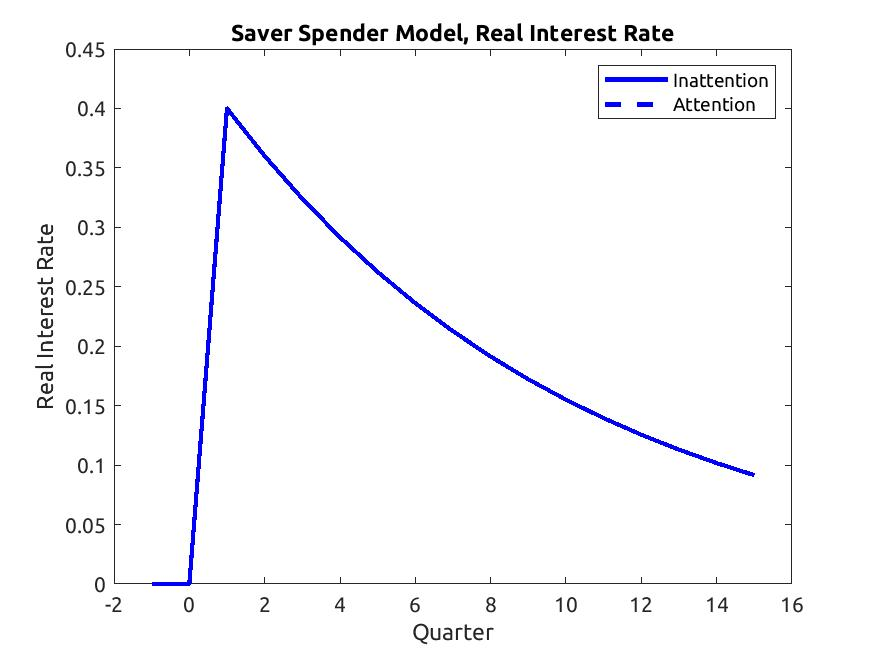
\includegraphics[width=0.45\textwidth]{../Code/Dynare/Figures/RealRateSS.jpg}
	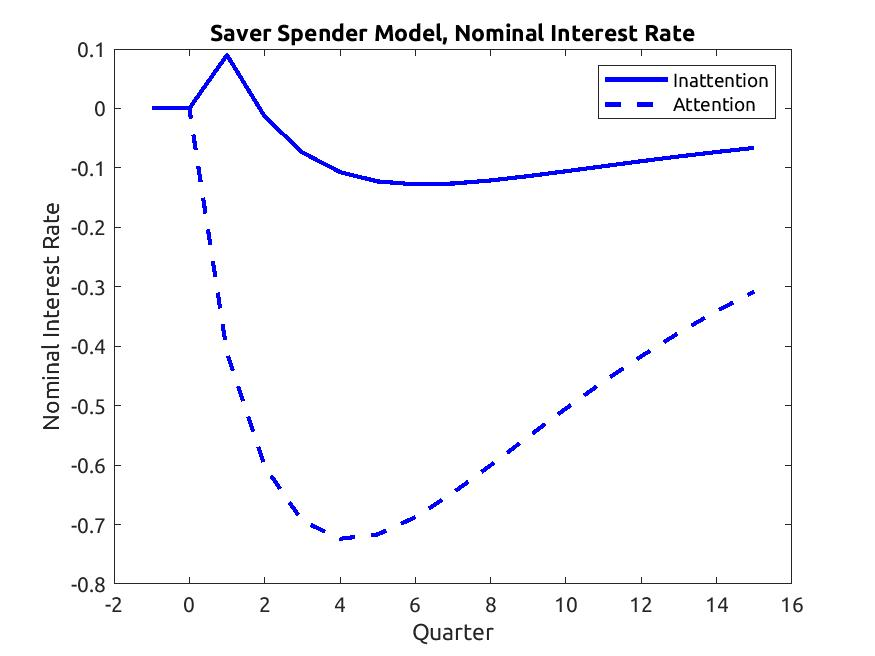
\includegraphics[width=0.45\textwidth]{../Code/Dynare/Figures/NominalRateSS.jpg}
	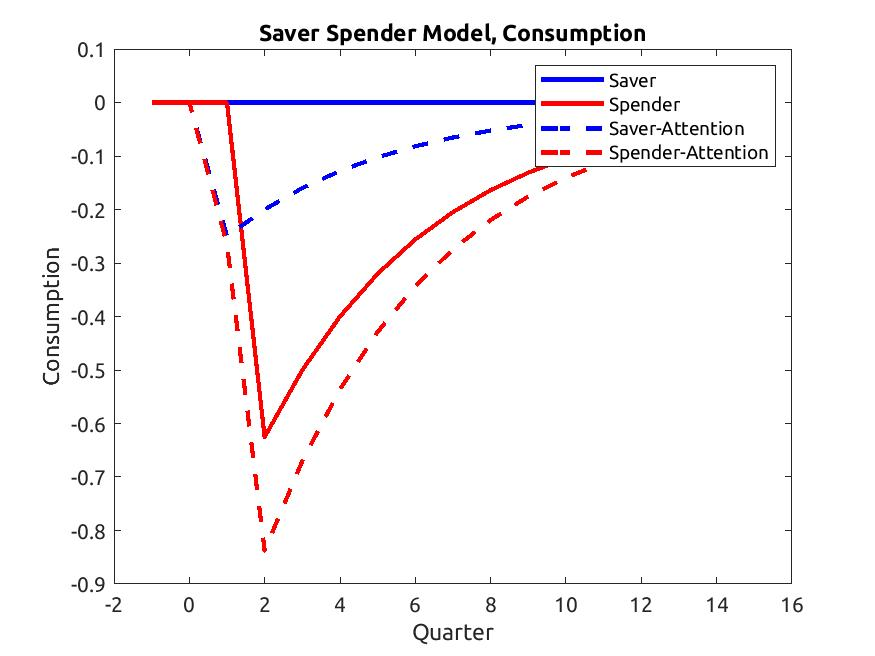
\includegraphics[width=0.45\textwidth]{../Code/Dynare/Figures/ConsumptionSS.jpg}
	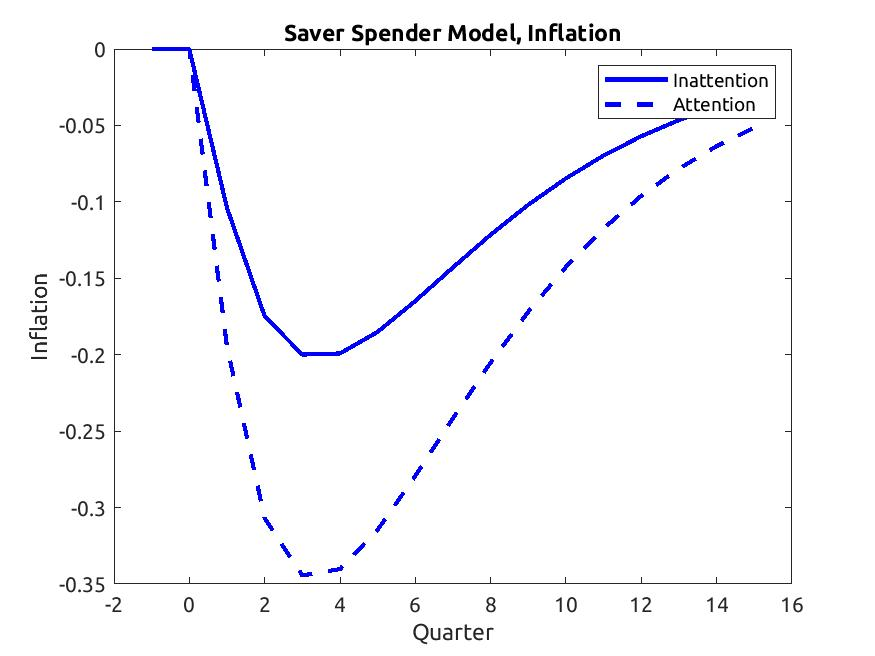
\includegraphics[width=0.45\textwidth]{../Code/Dynare/Figures/InflationSS.jpg}
	\caption{Impulse Response Functions to Saver Spender Model}
	\label{fig:IFRSS}
\end{figure}

Figure \ref{fig:IRFSS} shows the impulse response functions for this model under both attention and inattention to interest rates for the model in which the real rate is shocked directly. The lower-left panel on consumption for the two agent types is the most informative. The solid lines show the inattention version of the model. First, the saver in this model does not adjust consumption at all in response to the real interest rate change. Second, the spender adjusts consumption in the period after the shock when they have to pay a higher interest rate on their previous borrowing. The dashed lines show the model with attention. In this case, the saver adjust their consumption immediately on the interest rate news, and this reduces output which results in the spender also adjusting their consumption by the same amount. In the following period, the spender further reduces their spending as their budget constraint is hit with the higher interest rate, while the spender follows their Euler equation back to steady state.

\section{Model 2: An "Intertemporal MPC" Model}

One problem with the saver-spender model is that it assumes the spender has an MPC of one, so there is not much room for interesting dynamics in the model. We would like to have a realistic model for different agents intertemporal MPC, or "iMPC" from Auclert, Ronglie and Straub "Intertemporal Keynesian Cross". 

One simplification of assuming agents do not pay attention to interest rates in their Euler equation is that their iMPC now tells us what we need to know about their consumption response to interest rates, if we assume that changes in payments or receipts of interest are just like cash flow changes.

In the next model, we do not derive consumption behavior from a utility maximizing agent but instead write down behavior that is consistent with the empirical evidence we have for iMPCs. Under the assumption that agents don't pay attention to their Euler equations, this is sufficient to determine aggregate dynamics.

In the general version of this model, we can have several agents who have the following behavior with different parameters:
\begin{align}
	c_t = \text{mpc} (m_t + f_t)
\end{align}
where $c_t$ is the deviation in steady-state consumption, $\text{mpc}$ is the agent's MPC, $m_t$ is deviations in the agent's wealth and $f_t$ deviations in future wealth, which is possibly discounted heavily.

The state variables follow the law of motion:
\begin{align}
	m_t = a_{t-1}r_bar + n_t + \bar{A} r_{t-1}\\
	a_t = m_t - c_t
	f_t = \frac{1}{\Gamma} (n_{t+1} +\bar{A}r_t + f_{t+1} ) 
\end{align}
where $a_t$ is end-of-period assets and $\Gamma$ is the discounting applied to future cash flows. $\bar{A}$ is the steady state level of assets (or debt) held by this agent type. In aggregate, the sum of all assets is zero.

The specific model used makes use of two agents of this type, we'll call them saver and spender again. The saver has an MPC equal to $1-1/\bar{R}$ and $\Gamma=\bar{R}$, so their behavior is the same as the saver in the spender-saver model without attention. The `spender' has an MPC of 0.15 per quarter, and $\Gamma=\infty$ so that they discount future cash flows entirely. This fits with a fair amount of empirical evidence.

\begin{figure}
	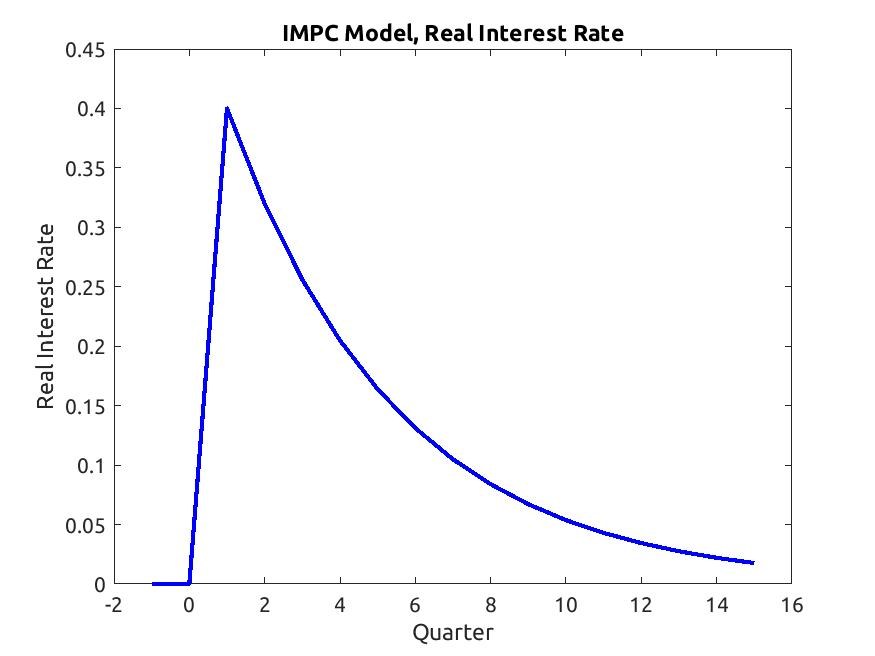
\includegraphics[width=0.45\textwidth]{../Code/Dynare/Figures/RealRateIMPC.jpg}
	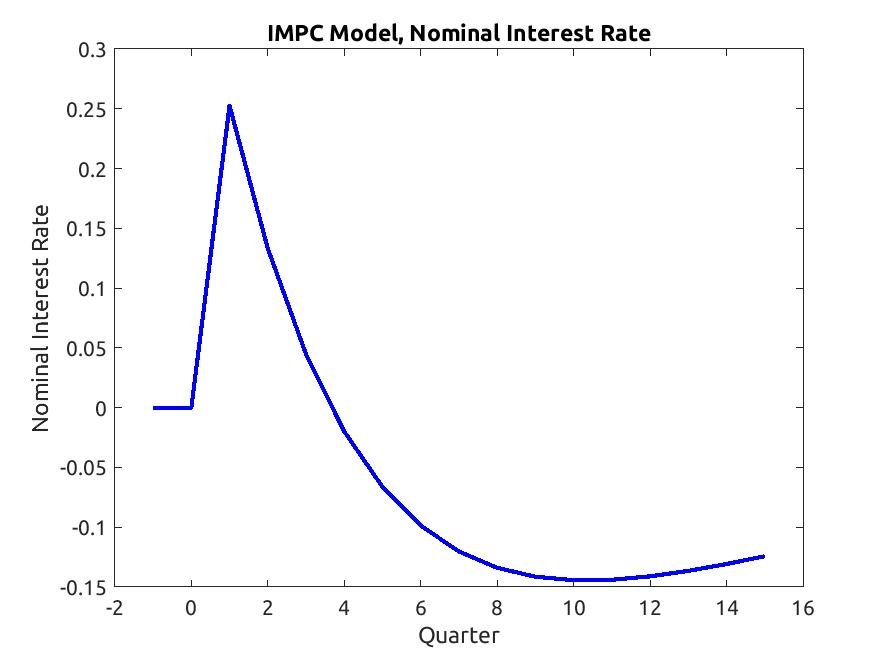
\includegraphics[width=0.45\textwidth]{../Code/Dynare/Figures/NominalRateIMPC.jpg}
	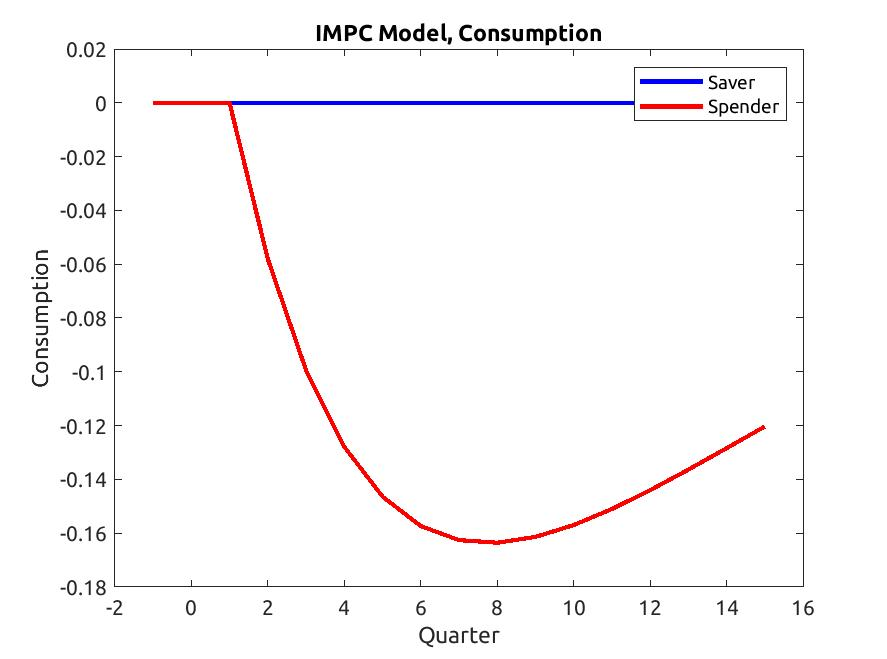
\includegraphics[width=0.45\textwidth]{../Code/Dynare/Figures/ConsumptionIMPC.jpg}
	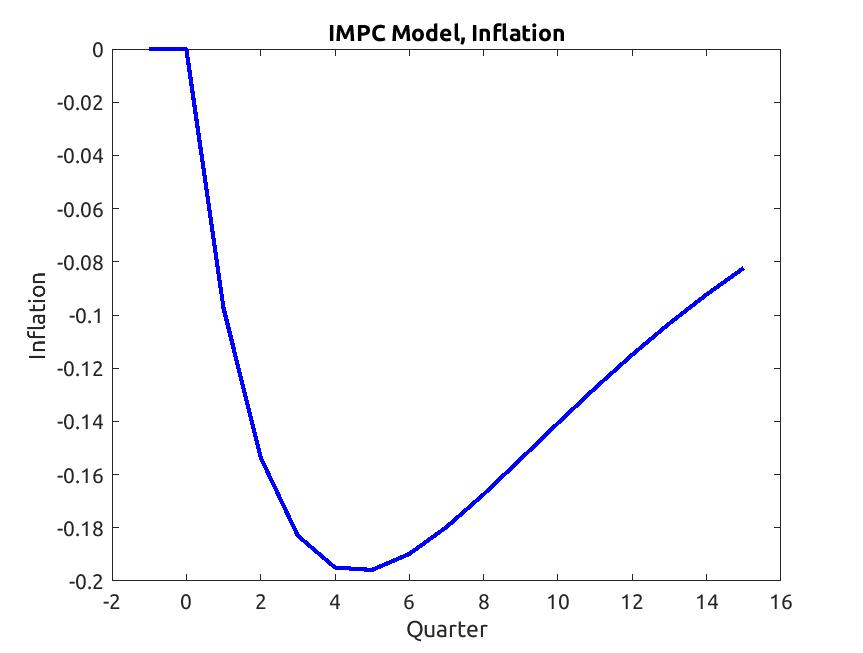
\includegraphics[width=0.45\textwidth]{../Code/Dynare/Figures/InflationIMPC.jpg}
	\caption{Impulse Response Functions to iMPC Model}
	\label{fig:IFRIMPC}
\end{figure}

Figure \ref{fig:IFRIMPC} shows the impulse response for this model. The real interest rate path is the same as in the saver-spender model, as is the consumption behavior of the `spender' who does not react to the shock. The key innovation in this model is the slow response of the `spender' consumption to the interest rate shock. While the real interest rate spikes up and then decays back to zero, the consumption of the spender reaches a peak 7 or 8 quarters out. This smoothed response is a result to two factors: i) the MPC is less than one, so the higher interest rate reduces spending both in the quarter it occurs and forward, and ii) the spenders do not react in advance to the fact they will expect lower cash flows in the future.

\section{Model 3: Long term debt}

Thus far, we have assumed the only available debt instrument is a one period bond.

In this long-term debt model, we assume a debt contract that pays exponentially decaying coupons. As with the saver-spender model, we assume the spender is able to borrow a fixed amount (in real terms) each period and will spend up to that limit. What they pay back the following period is then determined by the interest rate prevailing and each previous period.

The IRFs are shown in figure \ref{fig:IRFLT}. Here, although the spender has an MPC of one, the path of consumption is smoothed with the bottom 4 periods from the shock. This is despite the fact that the real interest rate peaks in period 1. The slow consumption response is because it takes time for the debt, most of which is fixed in period 1, the take on the new, higher, interest rate.
 
 
\begin{figure}
	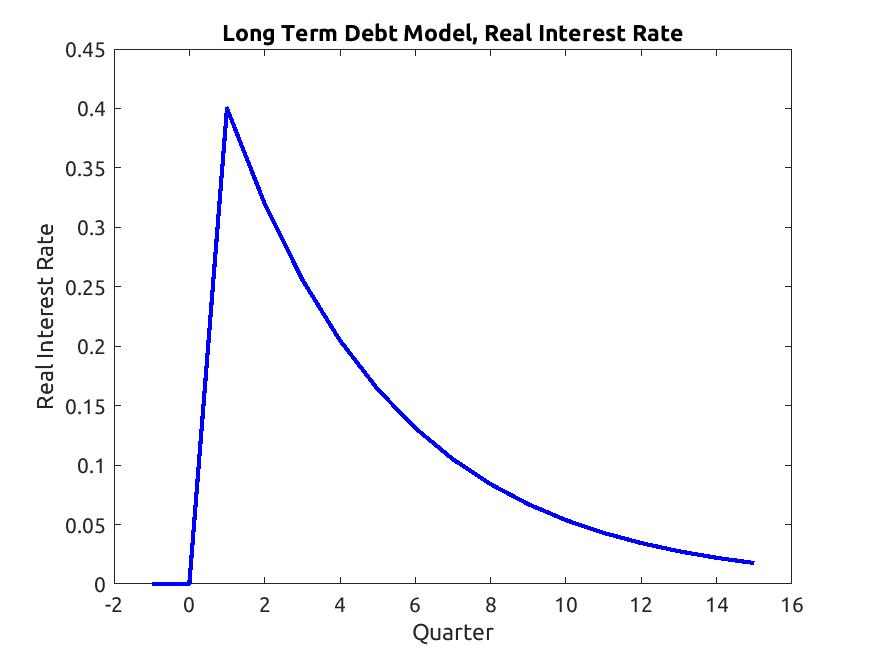
\includegraphics[width=0.45\textwidth]{../Code/Dynare/Figures/RealRateLT_debt.jpg}
	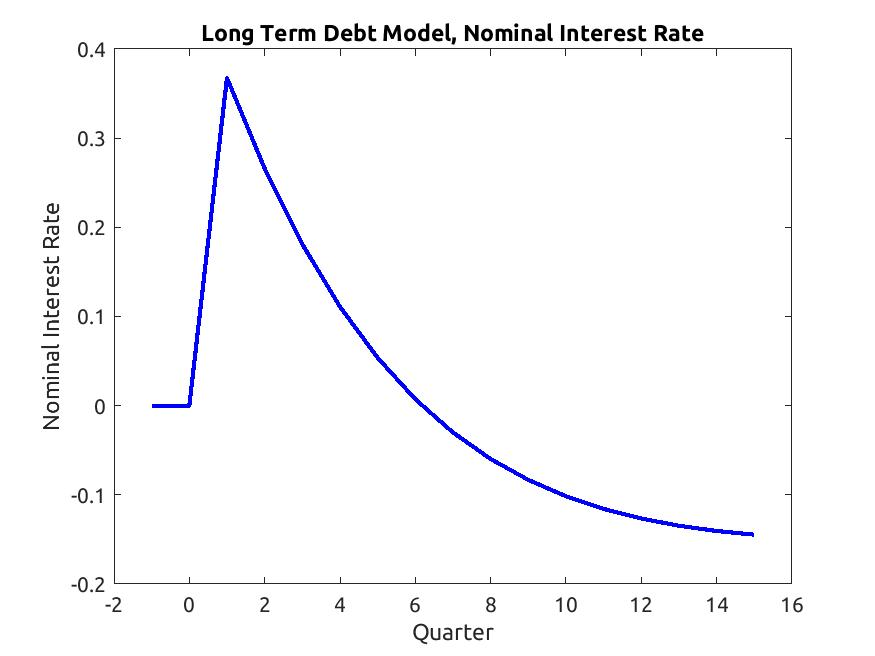
\includegraphics[width=0.45\textwidth]{../Code/Dynare/Figures/NominalRateLT_debt.jpg}
	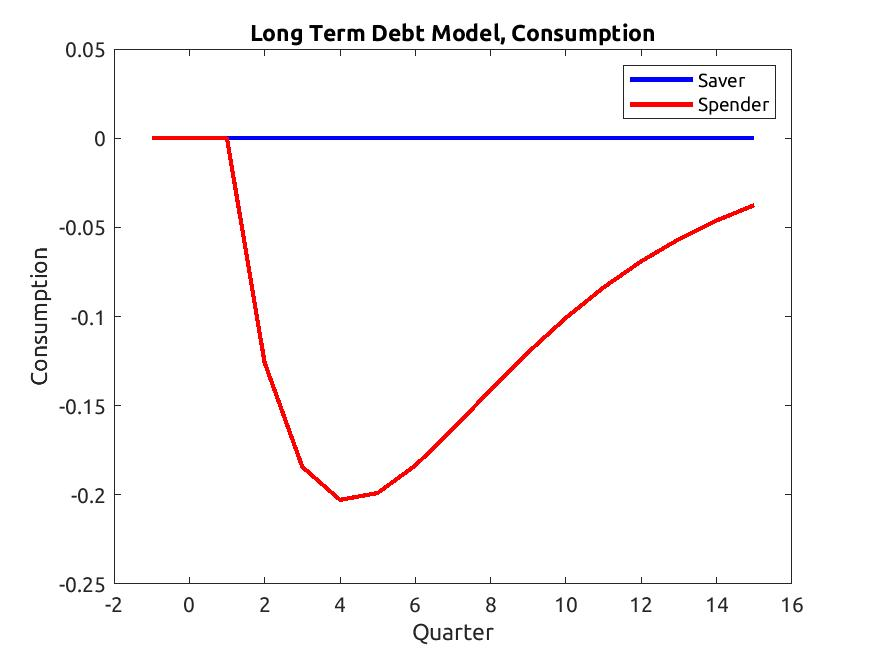
\includegraphics[width=0.45\textwidth]{../Code/Dynare/Figures/ConsumptionLT_debt.jpg}
	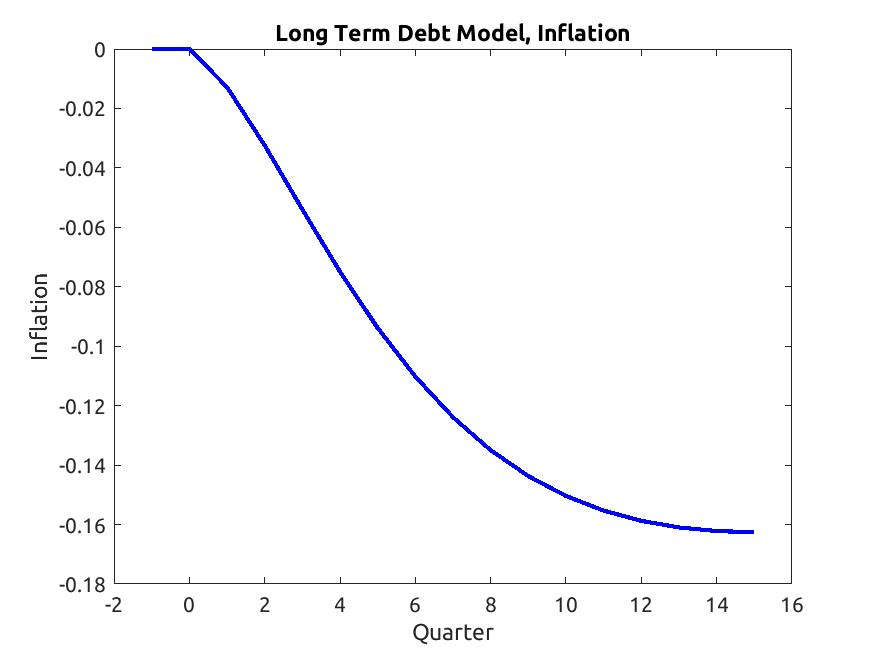
\includegraphics[width=0.45\textwidth]{../Code/Dynare/Figures/InflationLT_debt.jpg}
	\caption{Impulse Response Functions to Long term debt Model}
	\label{fig:IFRLT}
\end{figure}

\section{Thoughts}
No utility maximizing models can really rationalize the iMPCs we see in the data, so there is something to be said for the approach taken in Model 2. It would be good to mix Model 2 and Model 3, so that we have long term debt and more realistic iMPCs than an MPC of one.

TABU, or Two Agent Bonds in the Utility Function models are able to replicate empirical iMPCs fairly well. We might want to use these.

The way in which borrowing constraints are implemented can make a big difference, especially with longer-term debt. I have assumed in model 3 that you can borrow a fixed amount each period, regardless of your past commitments. This can be thought of as each period a certain amount of collateral becomes free to borrow against (e.g. you finance your car over 4 years).

To say something quantitative, I'd like to have a model of firms response to cash flows. Ultimately, consumers don't have enough debt to make this channel very large, but firms do. To some degree, we may be able to model firms in the same way as we do consumers in Model 2.

MPCs vary by type of income - changes in the value of a stock portfolio have a much lower consumption response than changes in labor income, even for the same individual. If we wanted to build a quantitative model, we would need to think about where the cash flow is going even within each individual (lower interest rates on mortgage $\rightarrow$ directly impact spending. Lower interest rates on bonds held in a pension $\rightarrow$ less so). Ultimately, most debt is held in pension accounts or by super rich individuals, or super well capitalized firms. 

There is also a difference in how mark-to-market differs between assets and debts. When interest rates rise, bond prices fall so bond holders are less wealthy. However, mortgage holders do not mark down the value of their mortgage.

All the models above abstract from financing of durables/houses.  We could apply this lens to the MoNK model of Garriga et al. \cite{garriga_monk_2019} or to Greenwald's JMP \cite{greenwald_mortgage_2018}. These papers inherit the fact that long term real rates are little changed by monetary policy, so their results are about monetary policy shocks to the long term inflation rate. I think our approach could give the CB more leverage over the real long term interest rate.



% Remove or comment out the next two lines if you are not using bibtex.
\bibliographystyle{aea}
\bibliography{WhoPaysAttention}

% The appendix command is issued once, prior to all appendices, if any.
\appendix

\end{document}

